$X_1$ is a complete graph and
\[
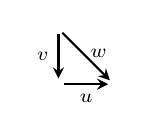
\begin{tikzpicture}[x=2em, y=2em, baseline=0.2em]
\begin{scope}[thick, -stealth, shorten >= 0.2em, shorten <= 0.2em]
\draw (0,1)--(0,0);
\draw (0,0)--(1,0);
\draw (0,1)--(1,0);
\end{scope}
\filldraw
(0,.5) node[anchor=east] {\scriptsize$v$}
(.5,0) node[anchor=north] {\scriptsize$u$}
(.4,.3) node[anchor=south west] {\scriptsize$w$};
\end{tikzpicture}
\Rightarrow\, \exists
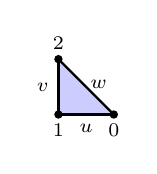
\begin{tikzpicture}[x=2em, y=2em, baseline=0.2em]
\filldraw[blue!20] (0,0)--(1,0)--(0,1);
\begin{scope}[thick]
\draw (0,1)--(0,0);
\draw (0,0)--(1,0);
\draw (0,1)--(1,0);
\end{scope}
\filldraw
(0,.5) node[anchor=east] {\scriptsize$v$}
(.5,0) node[anchor=north] {\scriptsize$u$}
(.4,.3) node[anchor=south west] {\scriptsize$w$}
(0,0) circle (1.3pt) node[anchor=north]{\scriptsize1}
(1,0) circle (1.3pt) node[anchor=north]{\scriptsize0}
(0,1) circle (1.3pt) node[anchor=south]{\scriptsize2};
\end{tikzpicture}
\]
